
% rubber: module pdftex

\documentclass[english,aspectratio=169]{beamer}
\usepackage{graphicx}
\usepackage{amssymb}
\usepackage{booktabs}
\usepackage{siunitx}
\usepackage{subcaption}
\usepackage{marvosym}
\usepackage[space]{grffile} % allows for spaces in filenames in \includegraphics

\newcommand{\pb}{\si{\pico\barn}}%
\newcommand{\fb}{\si{\femto\barn}}%
\newcommand{\invfb}{\si{\per\femto\barn}}

\newcommand{\GeV}{\si{\giga\electronvolt}}

\newcommand{\specialcell}[2][c]{%
  \begin{tabular}[#1]{@{}c@{}}#2\end{tabular}}

\newcommand{\beginbackup}{%
   \newcounter{framenumbervorappendix}
   \setcounter{framenumbervorappendix}{\value{framenumber}}
}
\newcommand{\endbackup}{%
   \addtocounter{framenumbervorappendix}{-\value{framenumber}}
   \addtocounter{framenumber}{\value{framenumbervorappendix}}
}

\usetheme[]{bjeldbak}

\begin{document}

\title[4t X-Section]{Four Tops X Section Measurement}
\subtitle{Trilepton Channel ($\mu^+\mu^-e, e^+e^-\mu$) }
\author[C. Fangmeier]{Caleb Fangmeier}
\institute[UNL]{University of Nebraska \-- Lincoln}
\date{\today}

\titlegraphic{%
\begin{figure}
  
\includegraphics[width=1in]{CMSlogo.png}\hspace{0.75in}
\includegraphics[width=1in]{nebraska-n.png}
\end{figure}
}

\begin{frame}[noframenumbering,plain]
  \titlepage%
\end{frame}

\section{Introduction}
\begin{frame}{Introduction}
  \begin{itemize}
    \item Beginning investigation of trilepton channel
    \item Specifically the $\mu^+\mu^-e, e^+e^-\mu$ final states
  \end{itemize}
\end{frame}


\begin{frame}{Decay Channels}
  The Decay channels are enumerated based on the types of W-decays
\begin{table}[]
  \tiny
  \begin{tabular}{@{}llccrrc@{}}
    \textbf{Name}               & \textbf{Leptons}           & \textbf{B-Jets} & \textbf{LF-Jets} & \textbf{BR}     & \textbf{BR ($\mu$ and $e$ only)} & \textbf{Events @ 40\invfb}    \\ \midrule
  Hadronic                    &                            & 4               & 8                & 20\%            & 20\%                             & 99                               \\ \midrule
  Single Lepton               & $\ell^\pm$                 & 4               & 6                & 40\%            & 26.6\%                           & 131                              \\ \midrule
  Same-Sign (SS) Dilepton     & $\ell^\pm \ell^\pm$        & 4               & 4                & 9.7\%           & 4.3\%                            & 21                               \\ \midrule
  Opposite-Sign (OS) Dilepton & $\ell^\pm \ell^\mp$        & 4               & 4                & 19.3\%          & 8.6\%                            & 42                               \\ \midrule
  Trilepton                   & $\ell^\pm\ell^\pm\ell^\mp$ & 4               & 2                & 9.8\%           & 2.9\%                            & 14                               \\ \midrule
  Leptonic                    & $\ell^+\ell^+\ell^-\ell^-$ & 4               & 2                & 1.2\%           & 0.24\%                           & 1                                \\ \bottomrule
  \end{tabular}
\end{table}
\vfill
\footnotesize{$\ell \in \left(e,\mu,\tau\right)$}
\end{frame}





\section{Strategy}

\begin{frame}{Strategy}
  \small
  \begin{itemize}
    \item Take advantage of the existing N-Tuples created by the TTH-Multilepton analysis
    \item Use the following baseline selection
    \begin{itemize}
      \item Exactly three charged leptons $\in(\mu^+\mu^-e, e^+e^-\mu)$
      \item Jet multiplicity $N_j \ge 4$
      \item B-Jet multiplicity $N_j \ge 3$
      \item Z-mass window veto: $M_{\ell^+\ell^-} \notin (70\GeV,105\GeV)$
    \end{itemize}
    \item Can then further breakdown into signal regions based on $N_j$ and other observables
  \end{itemize}
\end{frame}


\begin{frame}{Backgrounds (Irreducible)}
  \begin{center}
    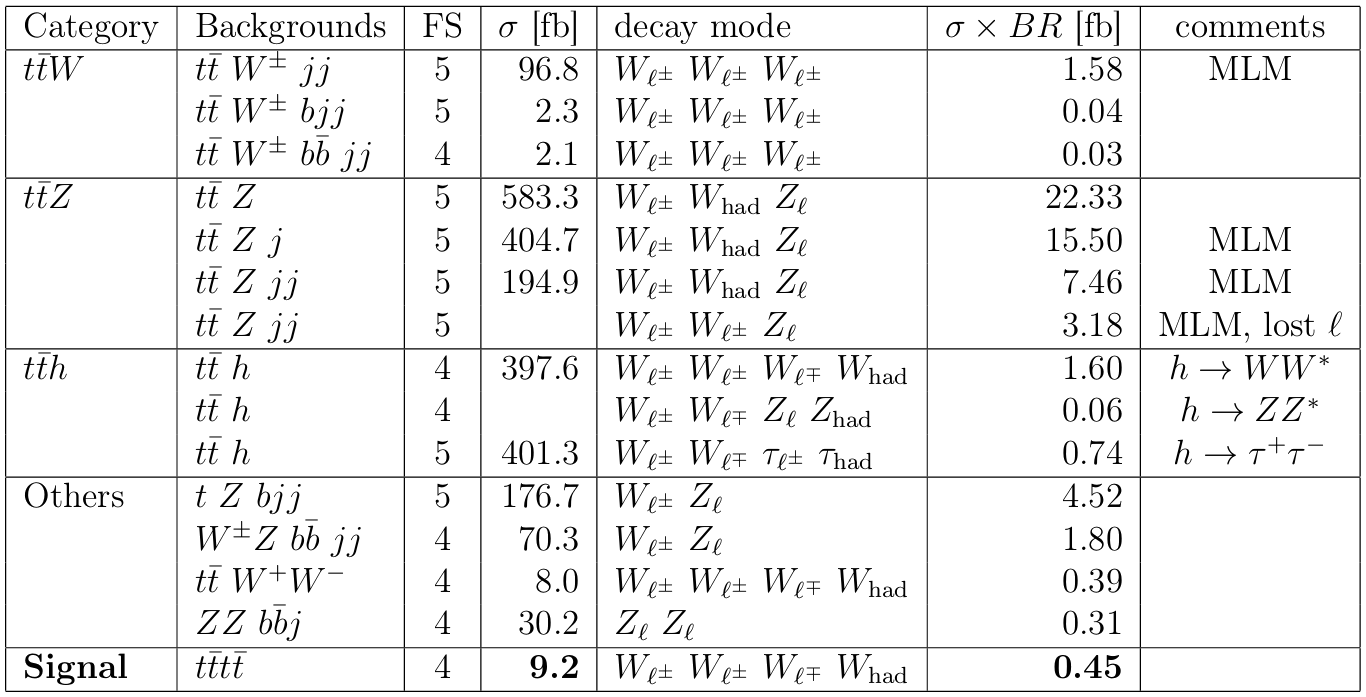
\includegraphics[width=0.8\textwidth]{figures/irreducible-backgrounds}
  \end{center}
\end{frame}


\begin{frame}{Backgrounds (Reducible)}
  \begin{center}
    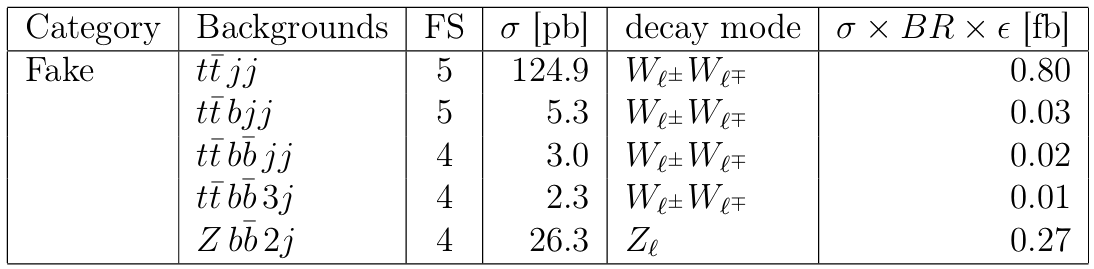
\includegraphics[width=0.8\textwidth]{figures/reducible-backgrounds}
  \\
  Here, $\epsilon=10^{-4}$, but will need to be corrected to measured value for CMS
  \end{center}
\end{frame}




\section{Some Preliminary Plots}

\newcommand{\rarrow}{$\rightarrow$}
\begin{frame}{Progress \& Status}
  \centering
  \footnotesize
  \begin{itemize}
    \item Acquired MC samples of signal and some relevant backgrounds
    \item Basic framework written to easily make distributions of N-Tuple variables as well as values derived from them. \\
      NTuple \rarrow{} (\texttt{filval} C++ Code) \rarrow{} \\
      Root File with Histograms \rarrow{} (Python plotting routines) \rarrow{} \\
      Plots in Jupyter Notebook
  \end{itemize}

  \tiny
  \begin{tabular}{ll}
  Sample Name                                                                                                    & X-section     \\
  /TTTT\_TuneCUETP8M1\_13TeV-amcatnlo-pythia8/RunIISummer16MiniAODv2-PUMoriond17\_80X\                           & 0.009103\pb{} \\
  \_mcRun2\_asymptotic\_2016\_TrancheIV\_v6-v1                                                                    &               \\
  /TTWJetsToLNu\_TuneCUETP8M1\_13TeV-amcatnloFXFX-madspin-pythia8/RunIISummer16MiniAODv2-PUMoriond17\_80X\       & 0.2043\pb{}   \\
  \_mcRun2\_asymptotic\_2016\_TrancheIV\_v6\_ext1-v3                                                              &               \\
  /TTZToLLNuNu\_M-10\_TuneCUETP8M1\_13TeV-amcatnlo-pythia8/RunIISummer16MiniAODv2-PUMoriond17\_80X\              & 0.2529\pb{}   \\
  \_mcRun2\_asymptotic\_2016\_TrancheIV\_v6\_ext1-v1                                                              &               \\
  /ttHJetToNonbb\_M125\_13TeV\_amcatnloFXFX\_madspin\_pythia8\_mWCutfix/RunIISummer16MiniAODv2-PUMoriond17\_80X\ & 0.215\pb{}    \\
  \_mcRun2\_asymptotic\_2016\_TrancheIV\_v6\_ext1-v1                                                              &               \\
  \end{tabular}
\end{frame}


\begin{frame}
  \centering
  % ROW 1
  \begin{minipage}[c][0.48\textheight]{0.32\textwidth}
      \includegraphics[width=\textwidth]{live_figures/Jet Multiplicity N_lep3.png}
  \end{minipage}
  \begin{minipage}[c][0.48\textheight]{0.32\textwidth}
    \includegraphics[width=\textwidth]{live_figures/Jet Multiplicity e+e-mu.png}
  \end{minipage}
  \begin{minipage}[c][0.48\textheight]{0.32\textwidth}
    \includegraphics[width=\textwidth]{live_figures/Jet Multiplicity mu+mu-e.png}
  \end{minipage}

  % ROW 2
  \begin{minipage}[c][0.48\textheight]{0.32\textwidth}
    \includegraphics[width=\textwidth]{live_figures/B-Jet Multiplicity N_lep3.png}
  \end{minipage}
  \begin{minipage}[c][0.48\textheight]{0.32\textwidth}
    \includegraphics[width=\textwidth]{live_figures/B-Jet Multiplicity e+e-mu.png}
  \end{minipage}
  \begin{minipage}[c][0.48\textheight]{0.32\textwidth}
    \includegraphics[width=\textwidth]{live_figures/B-Jet Multiplicity mu+mu-e.png}
  \end{minipage}
  \footnotesize
  Note that there is an overestimation of the jet counts as the lepton-tau-jet cross-cleaning still needs to be done.
\end{frame}


\section{Timeline}
\begin{frame}{Timeline}
  \begin{itemize}
    \item Target Graduation: Spring 2019
    \item $\rightarrow$ Primary Dataset 2016+2017(+top off with 2018)
    \item I have comps starting next week and running for the next month
  \end{itemize}
\end{frame}


\begin{frame}{References}
  \begin{itemize}
    \item \textbf{Analysis Code \& Results:}
      \url{https://tttt.fangmeier.tech}
  \end{itemize}
\end{frame}


\beginbackup%
\section{Backups}

\begin{frame}
  \huge
  \centering
  Backups
\end{frame}


\begin{frame}{Production}
  \begin{minipage}[c][\textheight]{0.45\textwidth}
    \begin{itemize}
      \item 4-top production can proceed through either
        \begin{itemize}
          \item<2,5-> $\mathcal{O}(\alpha_S^4)$ QCD Process
          \item<3,5-> $\mathcal{O}(\alpha_S^2 y_t^2)$ Higgs Exchange
          \item<4,5-> $\mathcal{O}(\alpha_S^2\alpha^2)$ Electroweak Process
        \end{itemize}
      \item<5-> Higgs Exchange + EW gives $\approx10\%$ contribution to total cross-section.
    \end{itemize}
  \end{minipage}
  \begin{minipage}[c][\textheight]{0.45\textwidth}
    \centering
    \only<2>{%
      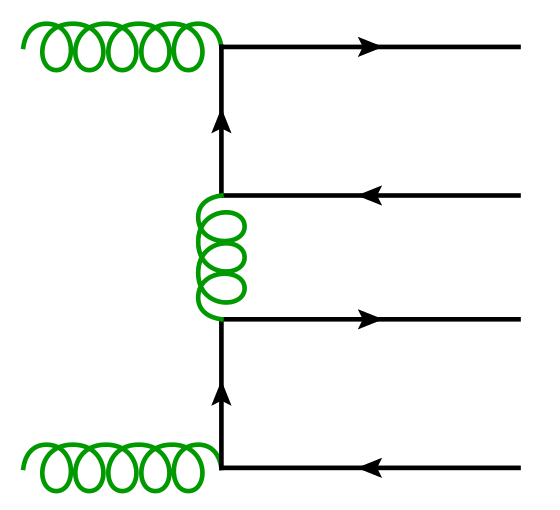
\includegraphics[width=\textwidth]{figures/production-qcd}
    }
    \only<3>{%
      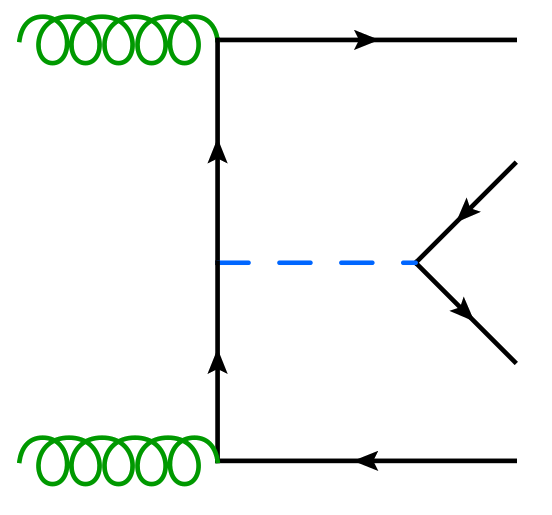
\includegraphics[width=\textwidth]{figures/production-higgs}
    }
    \only<4>{%
      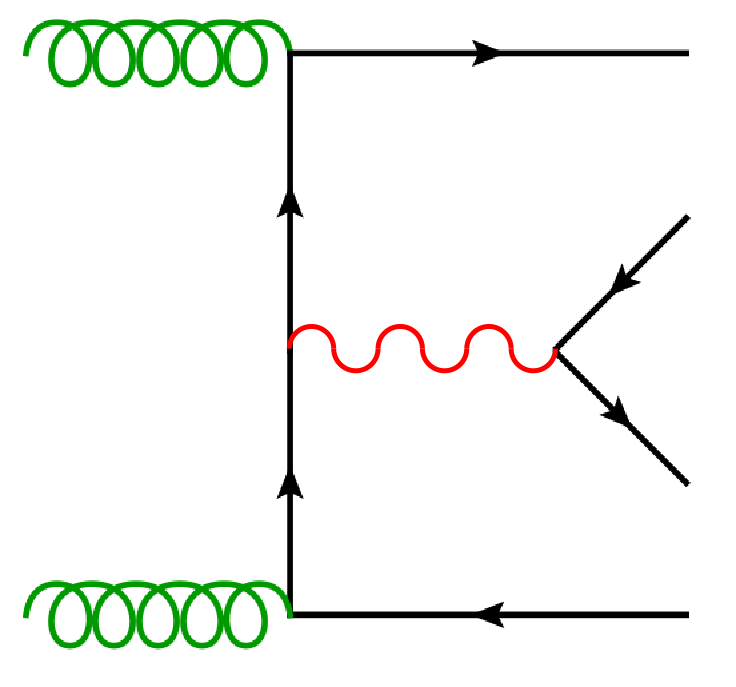
\includegraphics[width=\textwidth]{figures/production-ew}
    }
    \only<5>{%
      Standard Model cross-section at $\sqrt{s}=13\mathrm{TeV}$:
      \begin{center}
        \Huge{12.32\fb{} \MVAt{} NLO}
      \end{center}
    }
    \only<6->{%
      Standard Model cross-section at $\sqrt{s}=13\mathrm{TeV}$:
      \vspace{-.15in}
      \begin{center}
        \Large{12.32\fb{} \MVAt{} NLO}
      \end{center}
      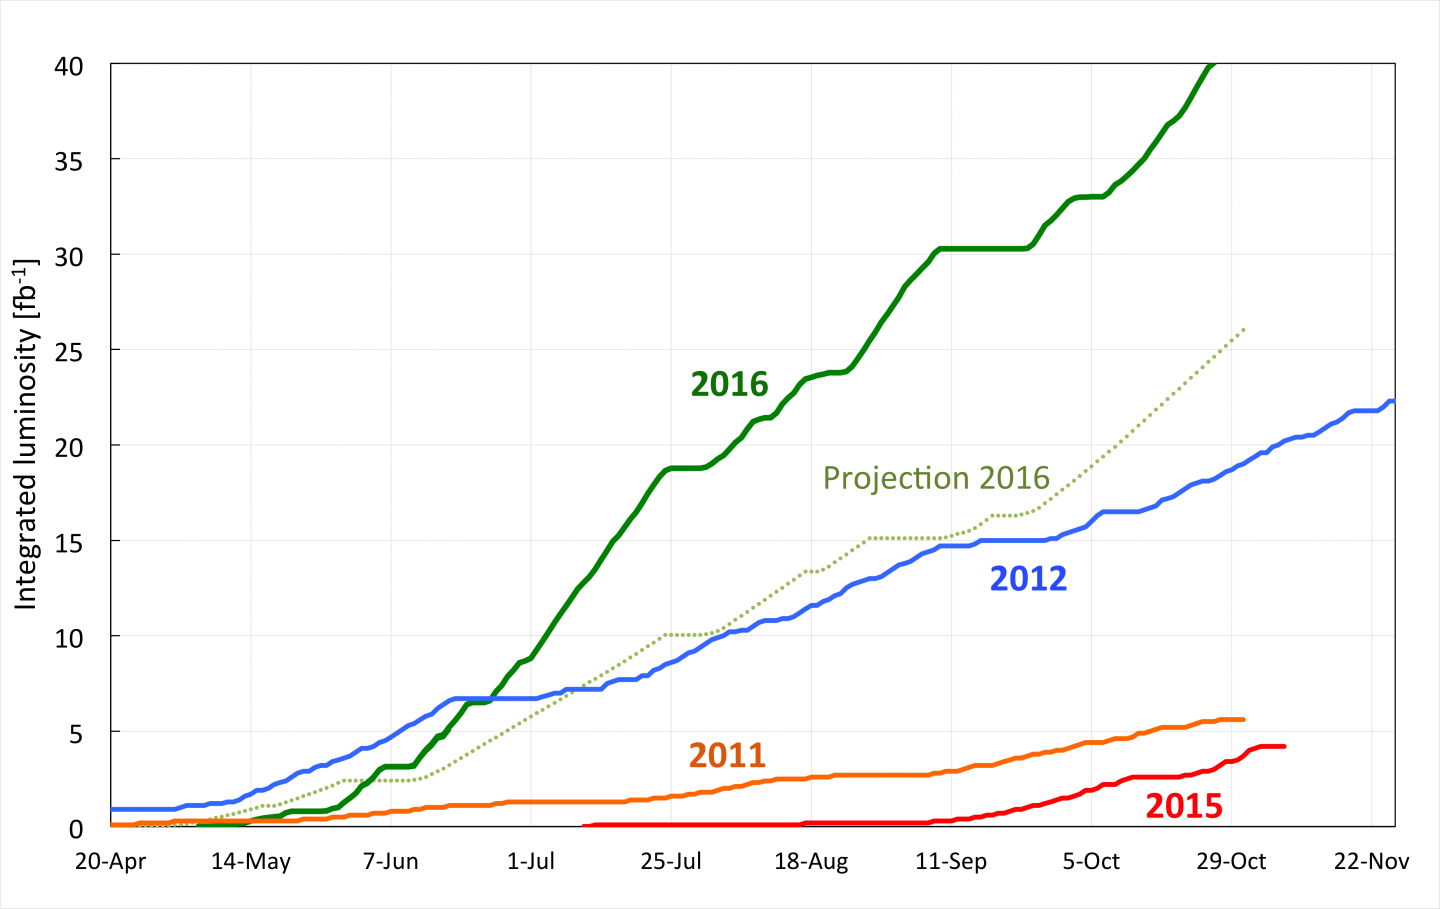
\includegraphics[width=\textwidth]{figures/lhc-luminosity-2016}
      % IMGSRC: https://home.cern/cern-people/updates/2016/12/lhc-report-far-beyond-expectations
      \vspace{-.15in}
      \begin{equation*}
        \mathrm{\#\ Signal\ Events}=12.32\fb * 40\invfb \approx 493
      \end{equation*}
    }
  \end{minipage}
\end{frame}


\begin{frame}{Decay Channels}
  \begin{minipage}[c][\textheight]{0.45\textwidth}
    \begin{itemize}
        %TODO: Check the limits on non-bW decays
      \item<1-> All* tops will immediately decay to a b-quark and a W-boson
      \item<2-> The W-boson will immediately decay either
        \begin{itemize}
          \item<2,4-> \textbf{Leptonically}
          \item<3-> \textbf{Hadronically}
        \end{itemize}
      \item<4-> The b-quark will form some b hadron, travel some macroscopic distance, and then hadronize into a jet.
    \end{itemize}
  \end{minipage}
  \begin{minipage}[c][\textheight]{0.54\textwidth}
    \centering
    \only<1>{%
      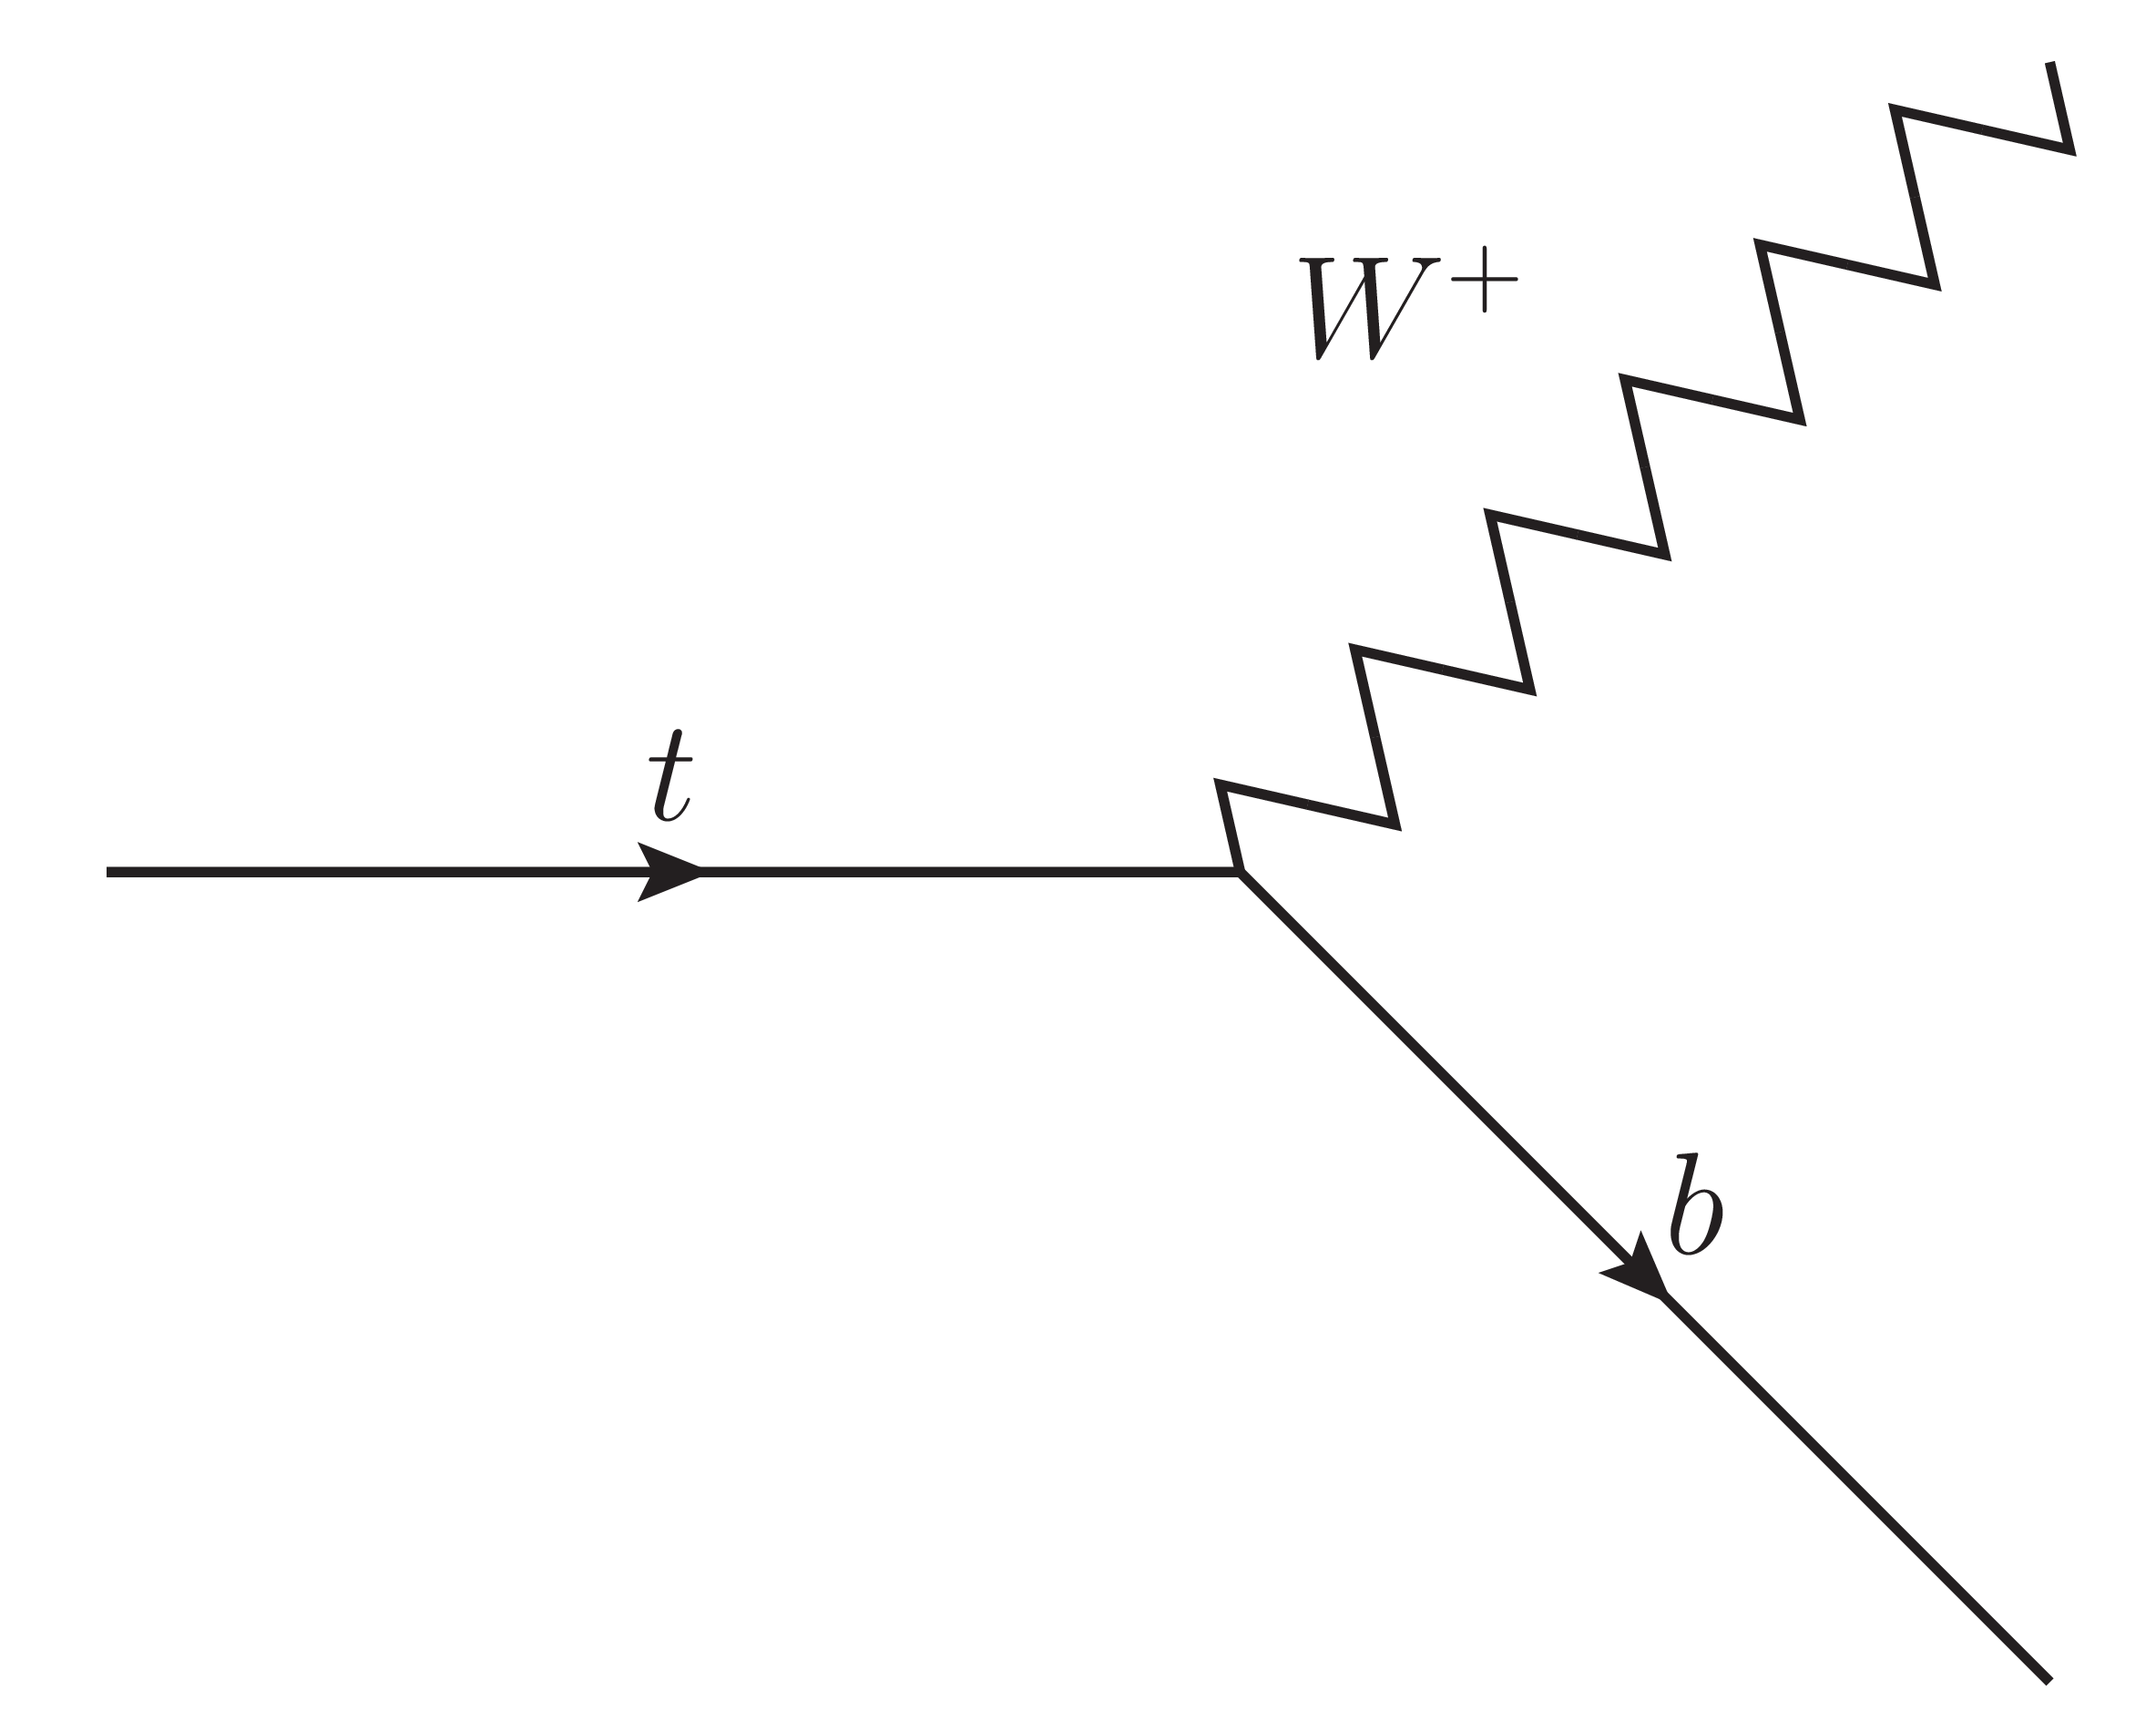
\includegraphics[width=\textwidth]{figures/feynman-diagrams/T-b_W.png}
    }
    \only<2>{%
      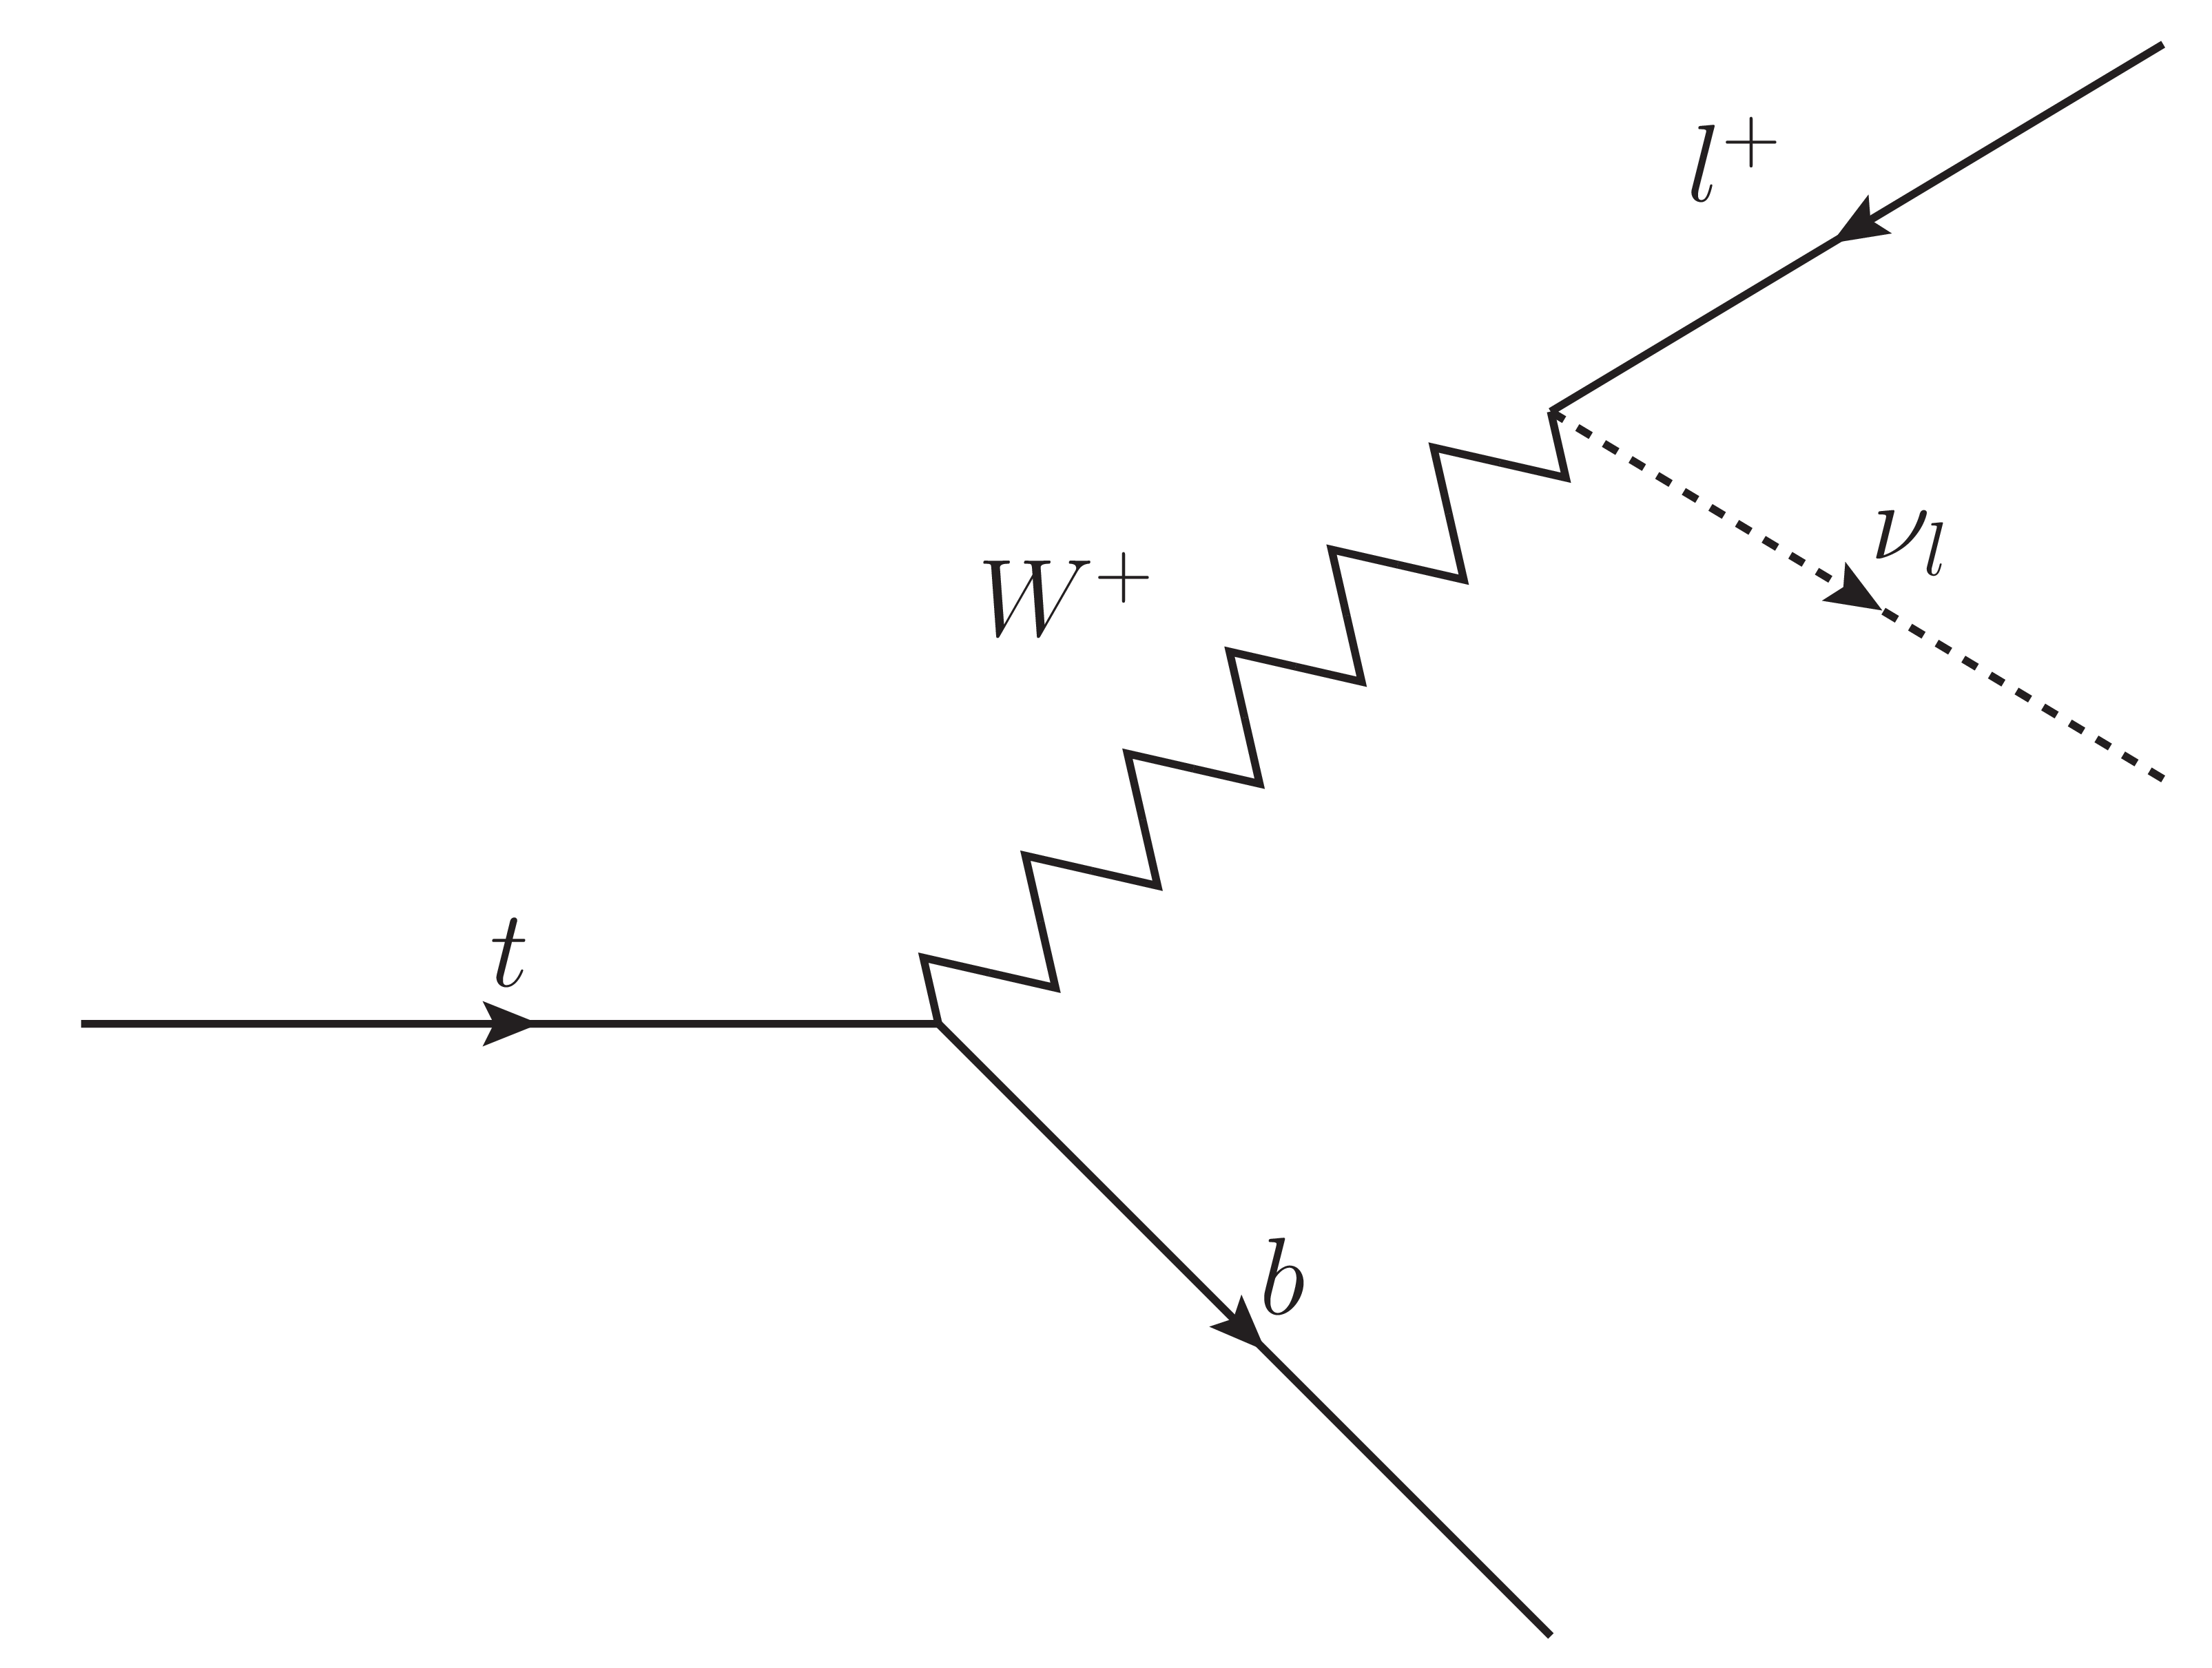
\includegraphics[width=\textwidth]{figures/feynman-diagrams/T-b_W-ln.png}
    }
    \only<3>{%
      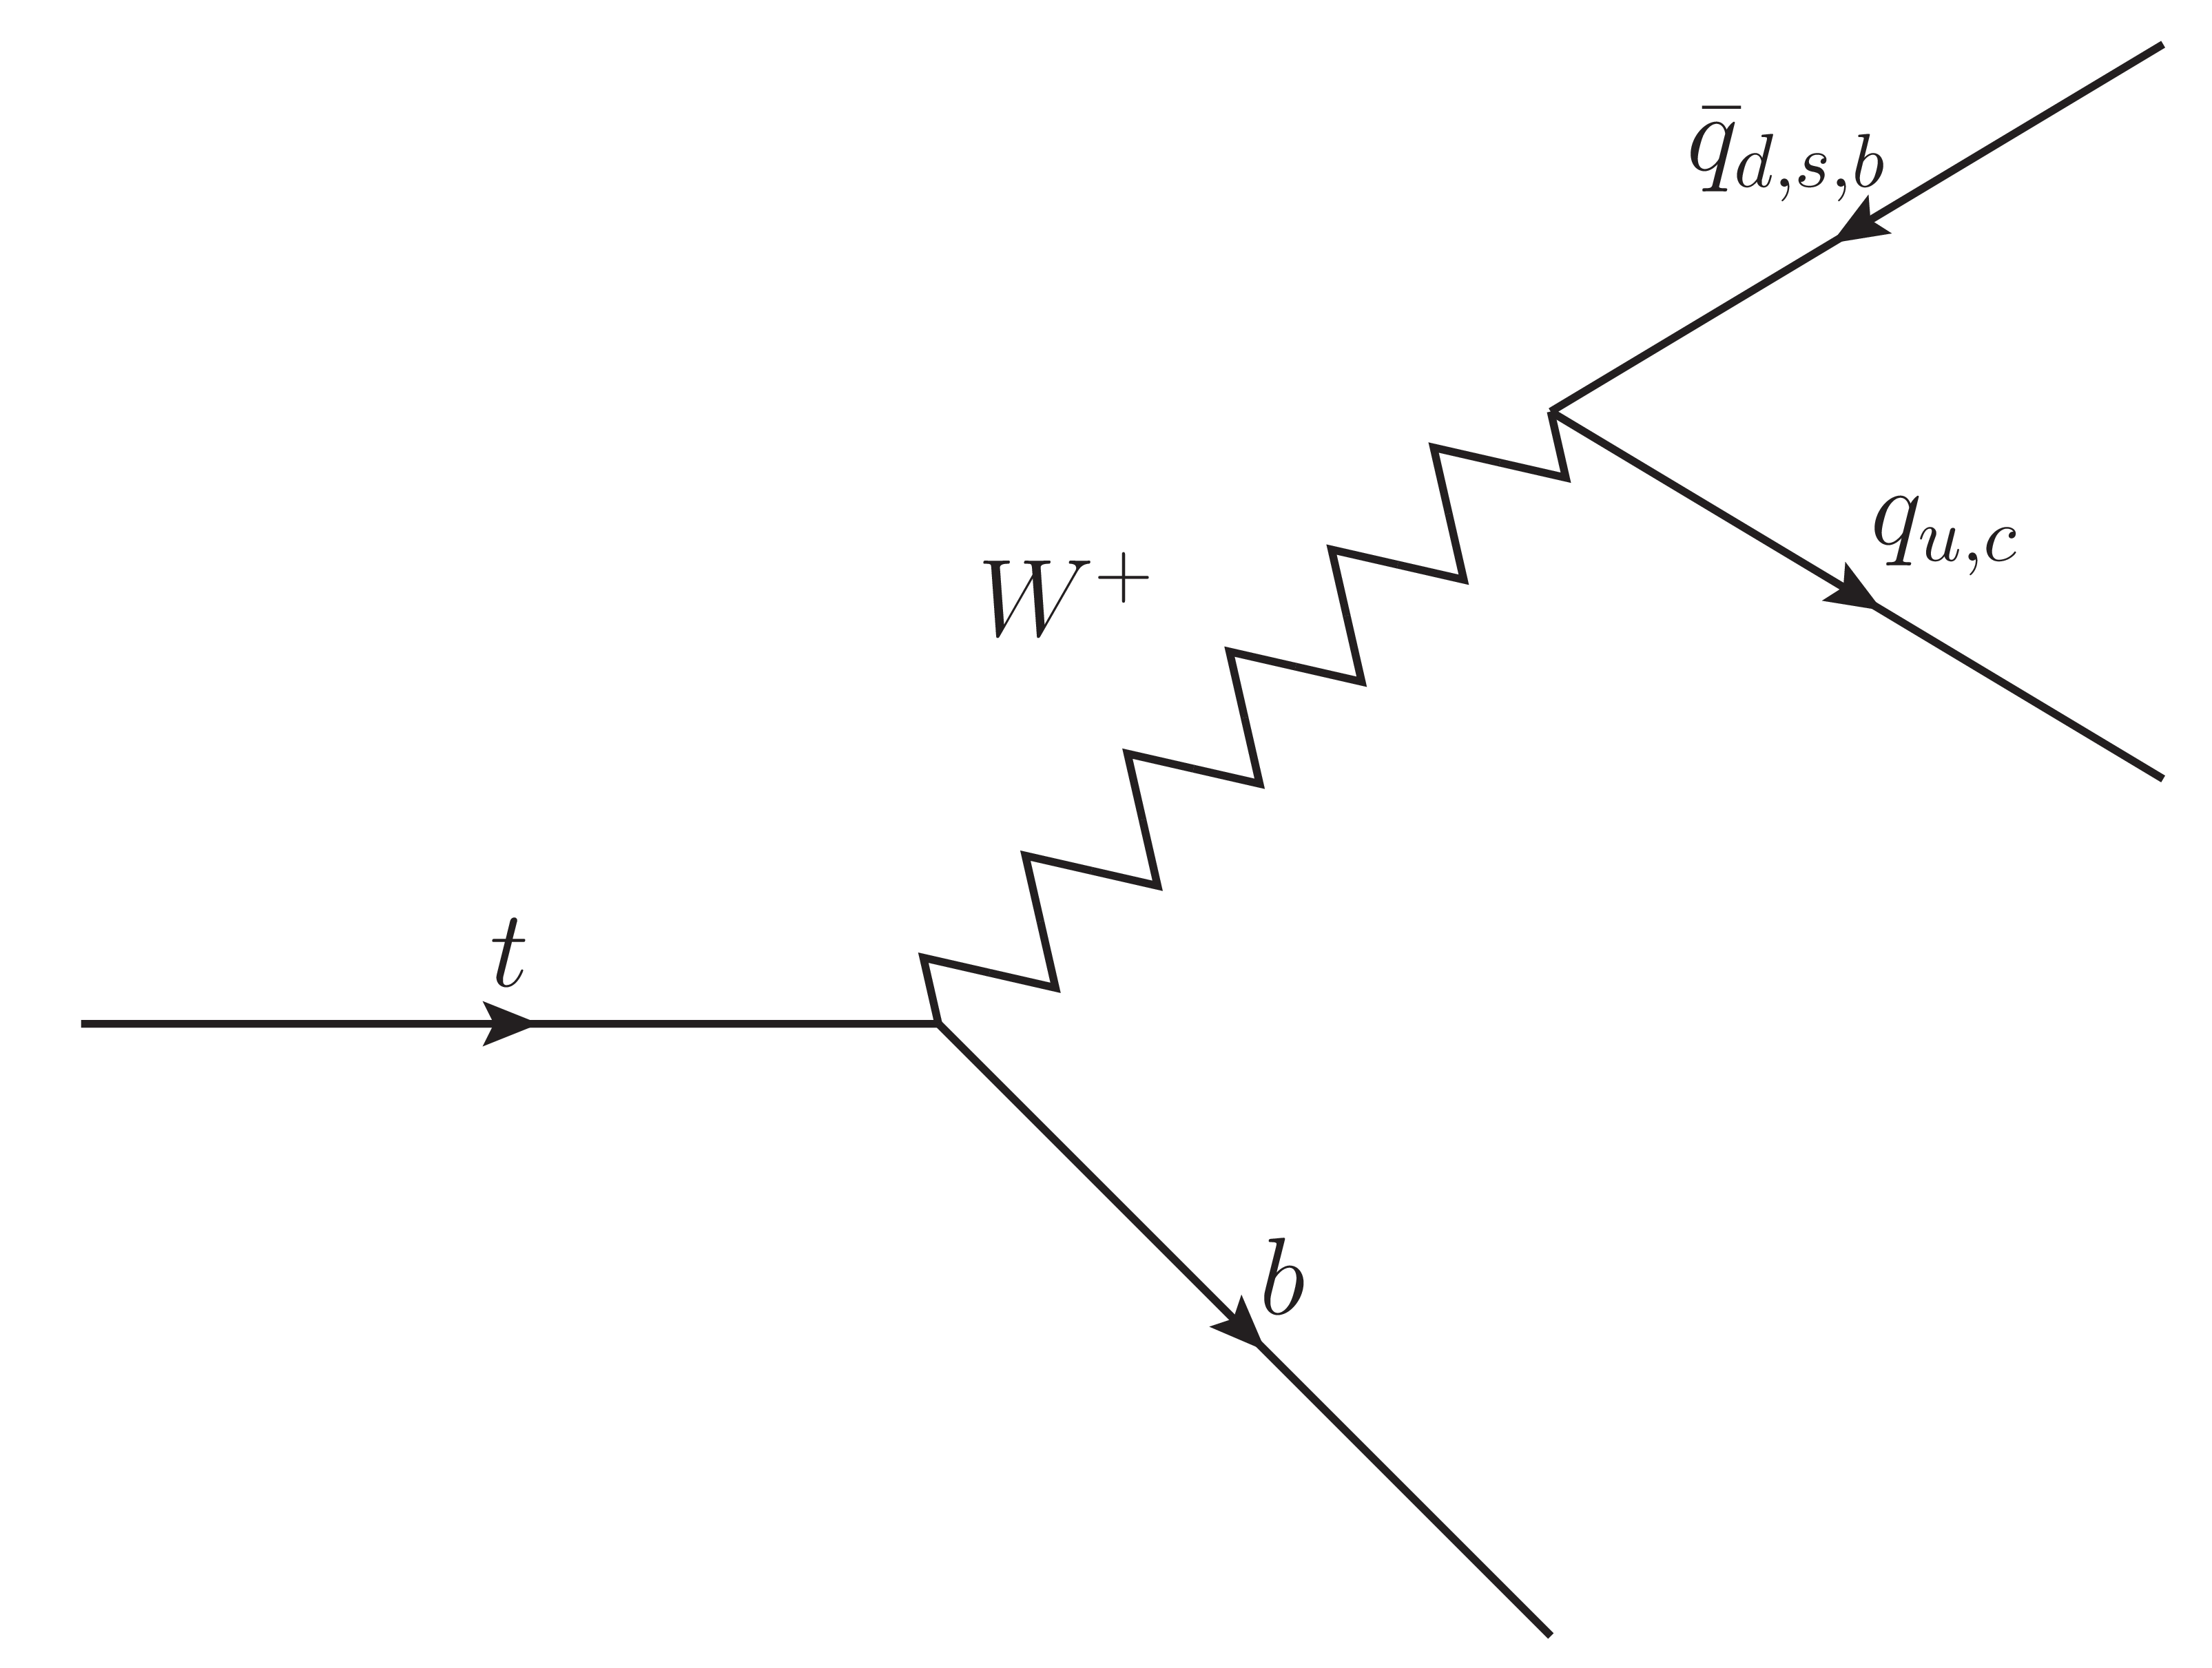
\includegraphics[width=\textwidth]{figures/feynman-diagrams/T-b_W-qq.png}
    }
    \only<4>{%
      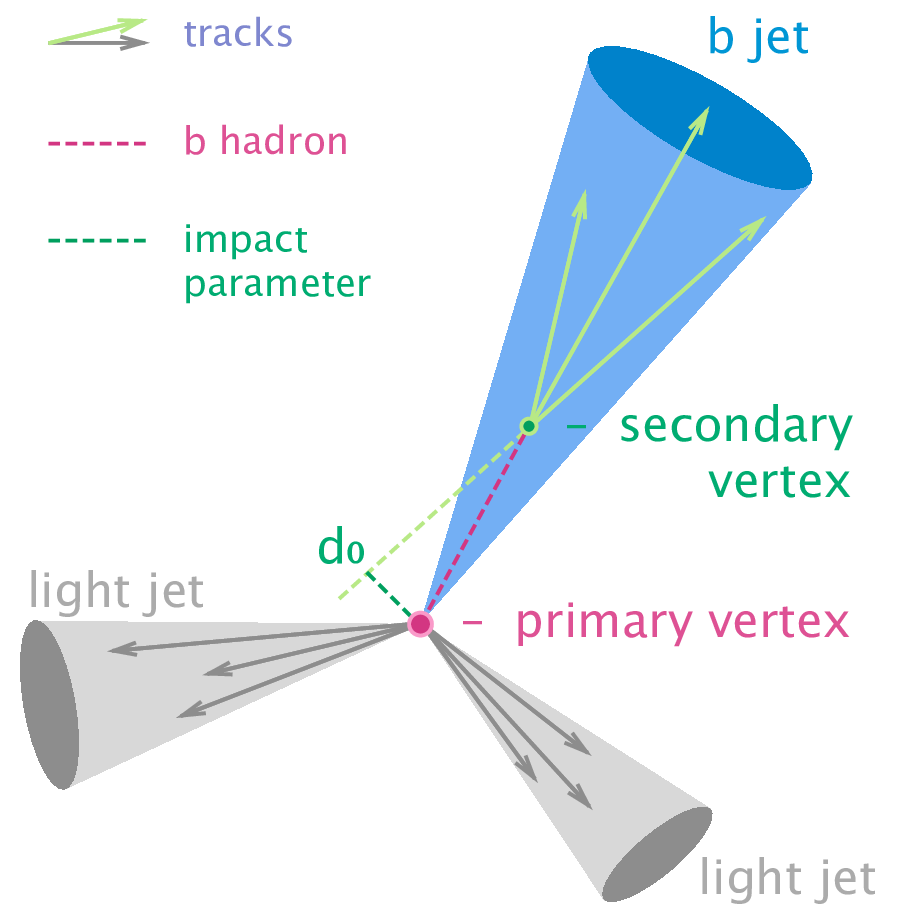
\includegraphics[width=0.90\textwidth]{figures/b-tagging}
    }
  \end{minipage}
\end{frame}


\begin{frame}{Previous CMS Measurements @ 13TeV}
\begin{table}[]
  \begin{tabular}{@{}lcr@{}}
  \textbf{Analysis}           & \textbf{Channel}            & \textbf{Limit}  \\ \midrule
  CMS-TOP-16-016              & Single Lepton, OS Dilepton  & 94\fb          \\ \midrule%
  CMS-SUS-15-008              & SS Dilepton                 & 119\fb         \\ \bottomrule%
  \textbf{Combined}           &                             & 69\fb          \\%
  \end{tabular}
\end{table}
\end{frame}


\endbackup%

\end{document}
